\section{Architecture générale de la solution}%
\label{sec.conception.archi}

Pour résoudre le problème de la réhabilitation de la parole aphasique,
nous proposons un système dont l'architecture générale est illustrée dans la Figure~\ref{fig.archi}.
Ce système est composé de deux parties principales :
\begin{enumerate*}[label=(\alph*)]
    \item le sous-système d'\gls{asr} qui permet de transcrire la parole aphasique en texte
    et dont l'architecture est illustrée dans la Figure~\ref{fig.asr-archi} et
    \item le sous-système de \gls{nmt} qui permet de traduire le texte transcrit en parole saine
    et dont l'architecture est illustrée dans la Figure~\ref{fig.nmt-archi}.
\end{enumerate*}

\begin{figure}[hbt]
    \begin{subfigure}{\textwidth}
        \begin{center}
            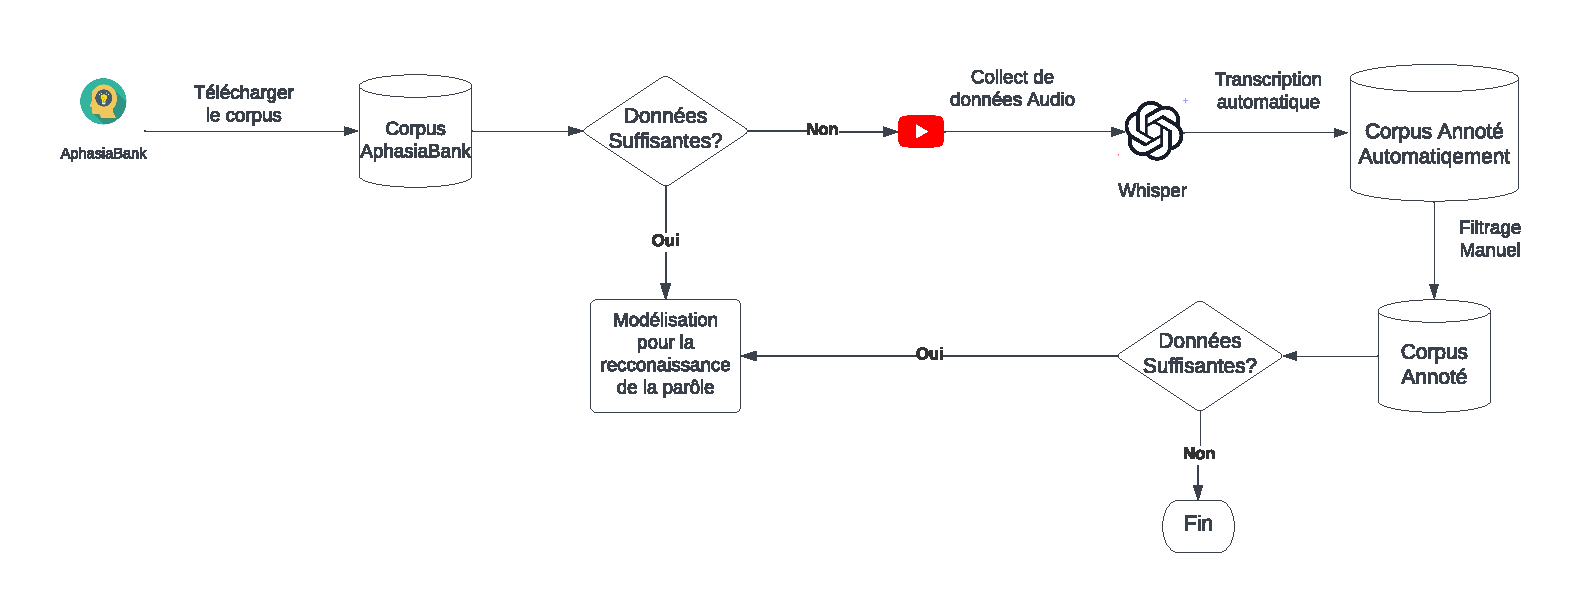
\includegraphics[height=6cm]{assets/pdf/ASR.pdf}
        \end{center}
        \caption{Déroulement de la partie \glsfmtshort{asr}.}
        \label{fig.asr-archi}
    \end{subfigure}
    %%
    \begin{subfigure}{\textwidth}
        \begin{center}
            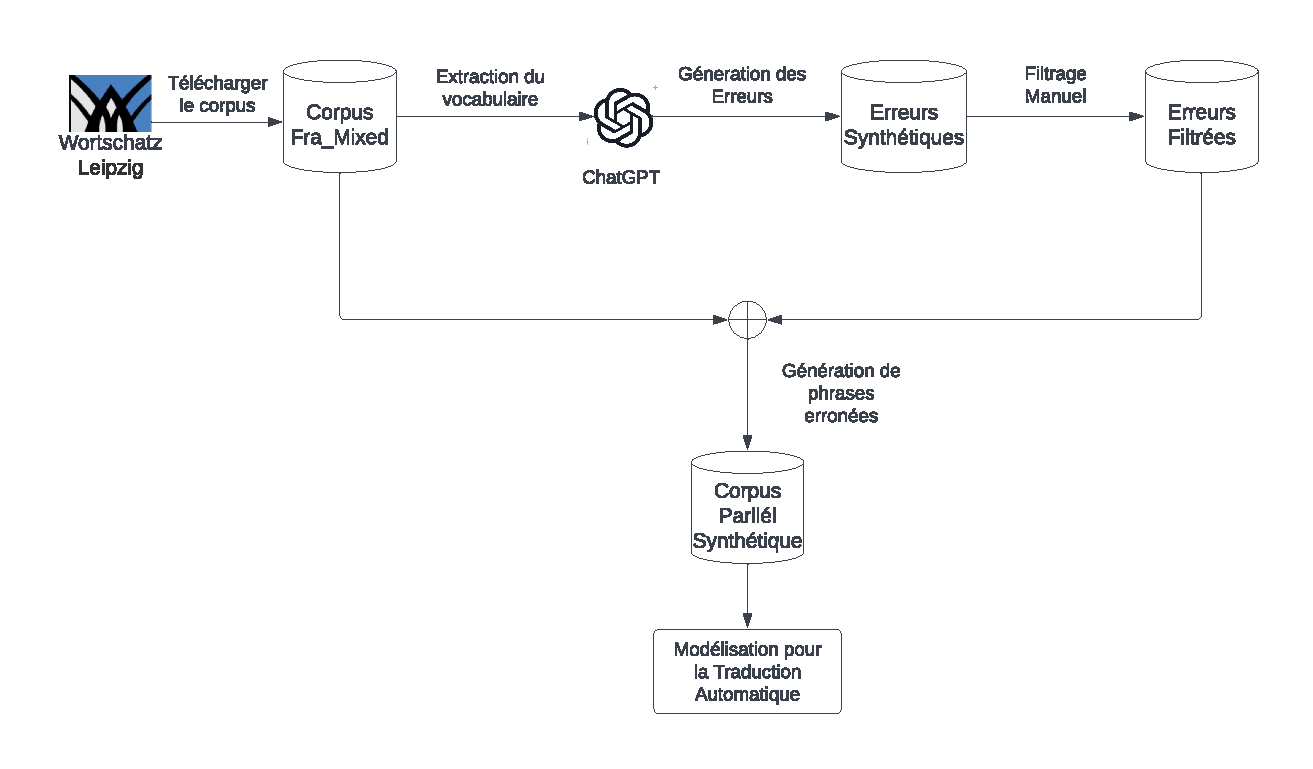
\includegraphics[height=8cm]{assets/pdf/NMT.pdf}
        \end{center}
        \caption{Déroulement de la partie \glsfmtshort{nmt}.}
        \label{fig.nmt-archi}
    \end{subfigure}
    %%
    \caption{Architecture générale de la solution.}
    \label{fig.archi} 
\end{figure}

Pour la partie \gls{asr}, nous avons choisi de l'organiser en deux activités principales :
\begin{enumerate}[label=(\roman*)]
    \item Préparation d'un corpus de donnée (parole/écrit), ce qui passe par :
    \begin{itemize}
        \item La collecte de données existantes : 
        consultation de corpus existants et de bases de données de parole aphasique,
        téléchargement et évaluation de ces données.
        Si les données collectées sont suffisantes (en qualité et en volume), 
        passer à la modélisation, sinon, passer à l'étape suivante.
        \item La collecte de données supplémentaires :
        repérage et téléchargement de vidéos de parole aphasique sur internet.
        \item Transcription des données collectées :
        dans un premier temps, les vidéos sont transcrites automatiquement à l'aide d'un modèle \gls{asr} existant.
        \item Filtrage manuel :
        les transcriptions automatiques sont filtrées manuellement pour corriger les erreurs de transcription.
        Le résultat de cette étape est un corpus de vidéos transcrites semi-automatiquement.
        \item Évaluation du corpus :
        si le corpus est suffisant (en qualité et en volume), 
        passer à la modélisation, sinon, passer à la partie \gls{nmt}.
    \end{itemize}
    \item Création et entraînement d'un modèle sur ce corpus.
\end{enumerate}

Une organisation similaire est adoptée pour la partie \gls{nmt} :
\begin{enumerate}[label=(\roman*)]
    \item Création d'un corpus parallèle (parole aphasique/parole saine) :
    contrairement à la partie \gls{asr}, aucun corpus parallèle n'est disponible pour l'aphasie de Broca.
    Dans l'absence de possibilité d'en créer un, nous avons choisi de créer un corpus parallèle synthétique.
    Cela peut être réalisé en suivant la procédure suivante :
    \begin{itemize}
        \item Prendre un corpus du Français.
        \item Extraire le vocabulaire de ce corpus.
        \item Sélection des mots : 
        choisir dans ce vocabulaire les mots qui sont \emph{``fréquents''} \emph{``difficiles''} à prononcer.
        \item Création des erreurs :
        passer ces mots au modèle chatGPT pour générer des variantes erronées.
        \item Filtrage manuel :
        traiter manuellement les erreurs générées pour ne garder que celles qui sont similaires aux erreurs produites dans l'aphasie de Broca.
        \item Création du corpus parallèle :
        à partir du corpus de l'original et des erreurs filtrées, créer un corpus parallèle.
    \end{itemize}
    \item Création et entraînement d'un modèle sur ce corpus :
    une fois le corpus parallèle créé, 
    il est possible de créer un modèle de traduction et de l'entraîner sur ce corpus.
    La démarche traditionnelle de \gls{dl} est suivie pour cette étape :
    \begin{itemize}
        \item Division du corpus :
        le corpus est divisé en trois parties :
        \begin{enumerate*}[label=\arabic*. ]
            \item corpus d'entraînement, utilisé pour entraîner le modèle,
            \item corpus de validation, utilisé pour évaluer le modèle pendant l'entraînement 
            et \item corpus de test, utilisé pour évaluer le modèle après l'entraînement.
        \end{enumerate*}
        \item Création du modèle :
        dans cette étape, l'architecture du modèle est choisie en fonction de la tâche en question.
        \item Entraînement du modèle :
        le modèle est entraîné sur le corpus d'entraînement pour ajuster ses paramètres.
        \item Évaluation du modèle :
        le corpus de test est utilisé pour mesurer la performance du modèle.
        Plusieurs métriques peuvent être utilisées pour cette évaluation.
        Si les résultats sont satisfaisants, passer à l'étape suivante, sinon, passer à l'étape précédente.
    \end{itemize}
\end{enumerate}

Dans la suite de ce chapitre, 
nous reprenons dans le détail les différentes étapes de cette architecture, 
que nous avons abordées brièvement dans cette section.

Une fois les deux modèles entraînés,
ils peuvent être enchainés pour former un système ``\foreignlanguage{english}{speech-to-speech}''
\begin{figure}[hbt]
    \begin{center}
        
\includegraphics[width=\textwidth]{assets/images/detail.png}
    \end{center}
    \caption{Système de réhabilitation de la parole aphasique.}
    \label{fig.sp2sp}
\end{figure}
\texttt{SA.mp3} représente le son aphasique,
la composante \gls{asr} du système permet de le transcrire en texte, produisant un texte aphasique \texttt{TA.txt}.
Ce texte est ensuite traduit en texte correct \texttt{TC.txt} par la composante \gls{nmt} du système.
Finalement, le texte correct est transformé en son correct \texttt{SC.mp3} par un outil de synthèse vocale.
